\section{Grundlegende Techniken}
Die Techniken, die im Bereich der nicht-photorealistischen Computergrafik 
eingesetzt werden, lassen sich in 3 Kategorien unterteilen:
\begin{itemize}
  \item im Geometrieraum
  \item im Projektionsraum
  \item im Bildraum.
\end{itemize}
  Im Geometrieraum wird das 3D-Modell der nachzubildenden Realität erzeugt, 
  dieses Modell wird dann über einen Betrachterblickpunkt in den 2D-Bildraum 
  projiziert. NPR-Techniken können in jeder der 3 Ebenen eingesetzt werden.

\subsection{Techniken im Geometrieraum}
Diese Art von Techniken übt direkten Einfluss auf die 3D-Geometrie eines Objektes 
aus. Nachteil dieser Technik ist jedoch der hohe Zeitaufwand bei der 
Manipulation und daher kommen diese Verfahren praktisch eher selten zum 
Einsatz. Techniken dieser Klasse sind zum einen "`Computer Sketching"', "`Noise 
Modifier"' und "`Level of Detail"'. Die Funktionsweise dieser Methoden wird im 
Nachfolgenden kurz vorgestellt.

\subsubsection{Computer Sketching}
Das "`Computer Sketching"' Verfahren wurde 1990 von Paul Bourk entwickelt. Er 
stellte sich die Frage, ob CAD-Anwendungen auch unscharfe, an menschliche 
Skizzen erinnernde Entwürfe ausgeben können. Dabei legte er folgende Kriterien 
für Skizzen fest: In Skizzen enden Linien nicht exakt an Kreuzungen 
(Schnittpunkten), sondern gehen über diese hinaus. Außerdem sind Linien nicht 
gradlinig sondern „verwackelt“. Diese Effekte erreichte Bourk durch die 
Manipulation des 3D-Modells, Linien wurden um einen zufälligen Faktor 
verlängert, gespalten und einer Mittelpunktverschiebung unterworfen.
\begin{figure}
  \centering
  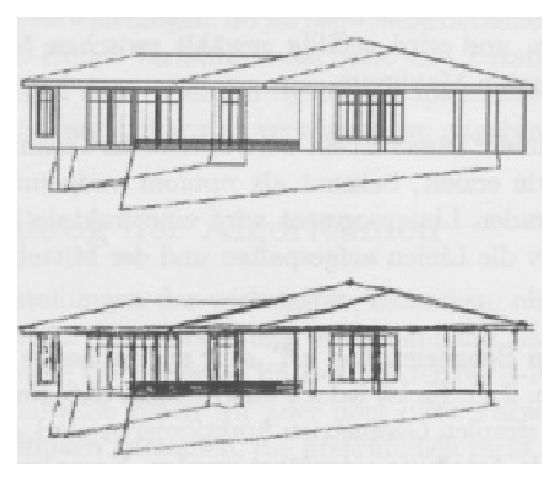
\includegraphics[width=0.60\textwidth]{../images/ComputerSketching}
  \caption{Oben Ausgabe ohne Computer Sketching, unten Ausgabe in der
  "`Sketchy"' Variante}
  \label{fig:ComputerSketching}
\end{figure}

\subsubsection{Noise Modifier}
In einer weiteren Technik im Geometrieraum kommen sogenannte Noise-Modifier zum 
Einsatz, diese erzeugen ein "`Rauschen"' in den 3D-Modellen. Dieses "`Rauschen"' 
wird erreicht, indem die Geometriepunkte der Flächen des Modells um einen 
zufälligen Faktor verschoben werden. Diese Verfahren finden hauptsächlich 
Anwendung auf glatte Flächen, um "`natürliche"' Flächen zu erzeugen.

\subsubsection{Level of Detail}
Ein Verfahren, das in vielen Bereichen Verwendung findet, ist das Level of 
Detail Prinzip, das unterschiedliche Detailstufen zur Darstellung nutzt. Es 
wird unter anderem in der Kartographie eingesetzt. Hier wird die Detailstufe in 
Abhängigkeit vom Maßstab der Karte dargestellt. Ein weiterer Einsatzbereich ist 
die photorealistische Computergrafik. Hier erfolgt die Darstellung der Details 
in Abhängigkeit von der Betrachterposition. Je näher ein Objekt dem Betrachter 
ist, desto genauer wird es dargestellt. NPR modifiziert dieses Prinzip und 
setzt die Detaillevel in Abhängigkeit zur "`Wichtigkeit"' der einzelnen Objekte. 
Je wichtiger ein Objekt für die Darstellung ist, desto genauer wird es 
dargestellt. Eine Möglichkeit zur Umsetzung bietet die Meshsimplifizierung. 
Hierbei wird die Anzahl der Polygone eines "`unwichtigen"' 3D-Modells reduziert 
und die äußere Form approximiert. Diese Technik unterstützt eine schnelle 
Verarbeitung und bietet so einen Einsatz in Echtzeitsystemen.

\subsection{Techniken im Projektionsraum}
Techniken im Projektionsraum werden meist mit Bildraumverfahren kombiniert, um 
ein leichteres Arbeiten mit 3D-Modellen und eine Erhöhung der grafischen 
Qualität der Ausgabe zu ermöglichen. Die Techniken arbeiten nach der Projektion 
und nutzen zusätzliche 3D-Informationen, wie Z-Werte oder Flächennormalen. 
Ein großer Vorteil dieser Techniken ist, wie oben schon angesprochen, die 
leichte Handhabung mit 3D-Modellen und daraus resultierend, die Erhöhung der
grafischen Qualität der Ausgabe. Ein Nachteil ist die komplizierte Berechnung
aufgrund der Verzerrungen. Verfahren, die im Projektionsraum Anwendung finden,
sind G-Buffer, Line-Rendering und Stroke Textures-Verfahren.

\subsubsection{G-Buffer}
Der G-Buffer (Saito u.\ Takahashi, 1990), ausgeschrieben "`Geometrie-Buffer"' 
genannt, ist in den meisten kommerziellen Cartoon-Render-Paketen implementiert. 
Das Prinzip basiert auf einer zusätzlichen Speicherung von geometrischen Daten 
zur Informationsgewinnung im Bildraum. So ist es beispielsweise möglich die 
Flächennormalen, die UV-Koordinaten oder die Z-Buffer-Werte eines 3D-Modells 
zusätzlich zu speichern, dies geschieht im Projektionsraum. Die Informationen 
werden dann für die Bilderzeugung aus dem G-Buffer extrahiert, analysiert und 
zusammengefügt.

\subsubsection{Line-Rendering}
Mit Hilfe der Line-Rendering Methode wird die Semantik von Linien simuliert. 
Dabei wird zwischen geometrischer und stilistischer Semantik unterschieden. 
Unter geometrische Semantik fallen Begrenzungen, Silhouetten, Diskontinuitäten 
und isoparametrische Konturen. Linienstärke, Transparenz und Linientyp 
(gestrichelt, durchgezogen, etc.) hingegen machen die stilistische Semantik 
aus. Im Projektionsraum werden für jede Linie die Charakteristiken, wie 
Wichtigkeit, Linientyp und Verdeckung, zum Beispiel mit Hilfe von 
Inferenzregeln bestimmt. Dann werden diese Attribute in geeigneter Form, etwa 
in Matrixform, abgespeichert und zur Bilderzeugung genutzt. Da sich diese 
Technik primär mit Linienstilen und ihren Semantiken beschäftigt, bietet sie 
eine gute Kombinationsmöglichkeit mit anderen NPR-Techniken, wie etwa mit dem 
zuvor vorgestelltem G-Buffer-Verfahren.

\subsubsection{Stroke Textures}
Das Prinzip der Stroke Textures (Winkenbach \& Salesin, 1994) basiert auf 
konventionellen 2D-Malsystemen. Es wird eine "`strichbasierte"' Textur 
angefertigt, die mittels Texturemapping auf bereits projizierte 3D-Objekte 
aufgebracht wird. Hierbei ist eine Anwendung des LOD-Prinzips auf die Textur 
möglich. Der Benutzer ist in der Lage die Linienstärke sowie sogenannte 
"`Detail Tags"' zu spezifizieren, um eine genauere Darstellung der Textur an 
ausgewählten Stellen zu erreichen.

\subsection{Techniken im Bildraum}
Bei Techniken im Bildraum geht man von einem vorhandenen Bild aus, das 
analysiert und neu "`gezeichnet"' wird. Vorteilhaft ist hierbei, dass das Bild 
bereits vorhanden ist, also keine Viewing-Pipeline nötig ist. Ein tragender 
Nachteil der Verfahren ist der, dass im Bildraum nur ungenauere Berechnungen 
möglich sind. Einige Verfahren, die im Bildraum angewendet werden, sind Texture 
Elements, Hairy Brushes und das Iterated Funktion System.

\subsubsection{Texture Elements}
Textur Elements (Mezei et al\., 1974) wurden ursprünglich zur Synthese sehr 
"`naturalistischer"' Bilder eingesetzt, da man in Beobachtungen festgestellt 
hatte, dass in der Natur sich wiederholende Muster vorkommen. Hierbei werden 
grafische Subelemente (größer als ein Pixel), die sogenannten "`Texture 
Elements"', vorgefertigt. Diese Elemente werden dann im eigentlichen 
Bilderzeugungsprozess zusammengefügt und ergeben so das neue Bild. Um 
Variationen im Bild zu erreichen, werden Skalierungen, Rotationen und andere 
Verzerrungen auf die Texture Elements angewendet. So werden Verallgemeinerungen 
der Oberflächeneigenschaften erzielt, die wie menschliche Illustrationen wirken.

\subsubsection{Hairy Brushes}
Mit dem Verfahren Hairy Brushes versuchte Strassmann 1986 als einer der ersten 
das Verhalten von Pinsel und Farbe zu simulieren. Der Pinsel wird dabei als 
1D-Abdruck seiner Borsten implementiert. Diese Borsten laufen an einer 
parametrisierten Kurve entlang, die durch Knoten definiert ist. Jeder dieser 
Knoten enthält Informationen über Position und Druck des Pinsels. Der Druck 
wird zwischen den Knoten interpoliert und gibt an, wie viel Farbe der Pinsel an 
den Zeichenuntergrund abgibt. Jeder "`Strich"' wird mit einer speziellen Menge 
an Farbe gezeichnet, die mit zunehmender Länge des "`Striches"' abnimmt. Die 
Farbe kann durch ein "`Eintunken"' des Pinsels wieder aufgefüllt werden, dies 
ermöglicht auch Variationen in der Farbe.

\subsubsection{Iterated Function System (IFS)}
Iterated Function System beschreibt ein System von Funktionen die wiederholt 
ausgeführt werden. Das System wird vor allem zur Beschreibung von Fraktalen 
eingesetzt. Fraktale sind selbstähnlich, d.\,h\. sie sind rekursiv aufgebaut. 
Eines der bekanntesten Beispiele ist der Barnsley-Farn. Der Rekursive Aufbau 
ist besonders gut in den Farnblättern zu erkennen (siehe Abbildung 
\ref{fig:BarnsleyFarn} und Abbildung \ref{fig:BarnsleyFarnDetail}).

\begin{figure}
  \centering
  \subfloat[Barnsley Farn]{
    
\includegraphics[width=0.3\textwidth]{../images/BarnsleyFarn.eps}
    \label{fig:BarnsleyFarn}
  }
  \qquad
  \subfloat[Barnsley Farn Detailansicht]{
    
\includegraphics[width=0.3\textwidth]{../images/BarnsleyFarnDetail.eps}
    \label{fig:BarnsleyFarnDetail}
  }
\end{figure}

Barnsley nutzte das Prinzip des IFS 1988 zur fraktalen Kompression von Bildern. 
Diese Kompressionstechnik basiert auf der Selbstähnlichkeit von Bildern, dem 
sogenannten "`Collage Theorem"'. Zwischen größeren und kleineren Teilen eines 
Bildes lassen sich bestimmte Ähnlichkeiten finden. Das zu komprimierende Bild 
(\ref{fig:IFS_Lena}) wird hierbei in "`range blocks"' unterteilt, dabei ist 
eine gleichmäßige Aufteilung möglich, wobei jeder Block im Allgemeinen eine 
Größe von 8x8 Pixeln besitzt. Aber auch eine Quadtree-Unterteilung ist denkbar, 
um Details besser wiedergeben zu können. (siehe Abbildung \ref{fig:Quadtree_Lena})

\begin{figure}
  \centering
  \subfloat[Lena]{
    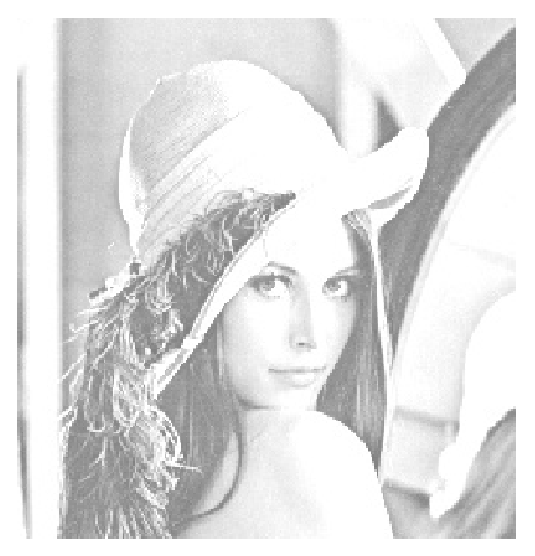
\includegraphics[width=0.4\textwidth]{../images/IFS_Lena.eps}
    \label{fig:IFS_Lena}
  }
  \qquad
  \subfloat[Quadtree-Unterteilung]{
    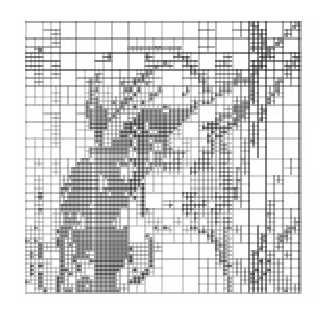
\includegraphics[width=0.45\textwidth]{../images/Quadtree_Lena.eps}
    \label{fig:Quadtree_Lena}
  }
\end{figure}